
% This LaTeX was auto-generated from MATLAB code.
% To make changes, update the MATLAB code and republish this document.

\documentclass{article}
\usepackage{graphicx}
\usepackage{color}

\sloppy
\definecolor{lightgray}{gray}{0.5}
\setlength{\parindent}{0pt}

\begin{document}

    
    
\section*{PIO Study for FDIR}


\begin{verbatim}Sam Nazari
16 Aug 2017\end{verbatim}
    
\subsection*{Contents}

\begin{itemize}
\setlength{\itemsep}{-1ex}
   \item Init Parameters and Dynamic System
   \item Observer dynamics
   \item Simulate Model
   \item Logging and Plotting
\end{itemize}


\subsection*{Init Parameters and Dynamic System}

\begin{verbatim}
clear
clc
Tsim = 5;

% create the dynamic system structure
A = [-1 1;0 -2];
B = [0;1];
C = eye(2);
D = 0;
E = [0;1];

sys = ss(A,B,C,D);

% create initial conditions
X_0 = zeros(2,1);
% observer initial conditions
XI_0= zeros(2,1);
xY_0= rand(2,1);
Xhat_0 = rand(2,1);
\end{verbatim}


\subsection*{Observer dynamics}

\begin{verbatim}
Ax = [A B; 0 0 0]
Bx = [B;0]
Cx = [C zeros(2,1)]

sysObs = ss(Ax,Bx,Cx,0)

[Lx prec] = place(Ax',Cx',[-10,-20,-30])
Lx = Lx'
Lp = Lx(1:2,1:2)
Li = Lx(3,1:2)
Ao = Ax-Lx*Cx;
Ap = A-Lp*C;
\end{verbatim}

        \color{lightgray} \begin{verbatim}
Ax =

    -1     1     0
     0    -2     1
     0     0     0


Bx =

     0
     1
     0


Cx =

     1     0     0
     0     1     0


sysObs =
 
  A = 
       x1  x2  x3
   x1  -1   1   0
   x2   0  -2   1
   x3   0   0   0
 
  B = 
       u1
   x1   0
   x2   1
   x3   0
 
  C = 
       x1  x2  x3
   y1   1   0   0
   y2   0   1   0
 
  D = 
       u1
   y1   0
   y2   0
 
Continuous-time state-space model.


Lx =

   19.0225   -0.9257  -12.0730
    0.6517   37.9775  299.8728


prec =

    15


Lx =

   19.0225    0.6517
   -0.9257   37.9775
  -12.0730  299.8728


Lp =

   19.0225    0.6517
   -0.9257   37.9775


Li =

  -12.0730  299.8728

\end{verbatim} \color{black}
    

\subsection*{Simulate Model}

\begin{verbatim}
sim('PIOModel')
\end{verbatim}

\includegraphics [width=4in]{PIO_init_01.png}


\subsection*{Logging and Plotting}

\begin{verbatim}
e = logsout;
er= e{1}.Values.Data;
t = e{1}.Values.Time;

set(groot, 'defaultAxesTickLabelInterpreter','latex'); set(groot, 'defaultLegendInterpreter','latex');
figure(1)
plot(t,er(:,1),'b',t,er(:,2),'r','LineWidth',2),xlabel('Time (sec)'), ylabel('State Estimation Error')
title('State Estimation Error'), grid on
xlim([0 1])
ylim([-0.5 0.5])
legend(['x_1 - xHat_1'],['x_2 - xHat_2'])
\end{verbatim}

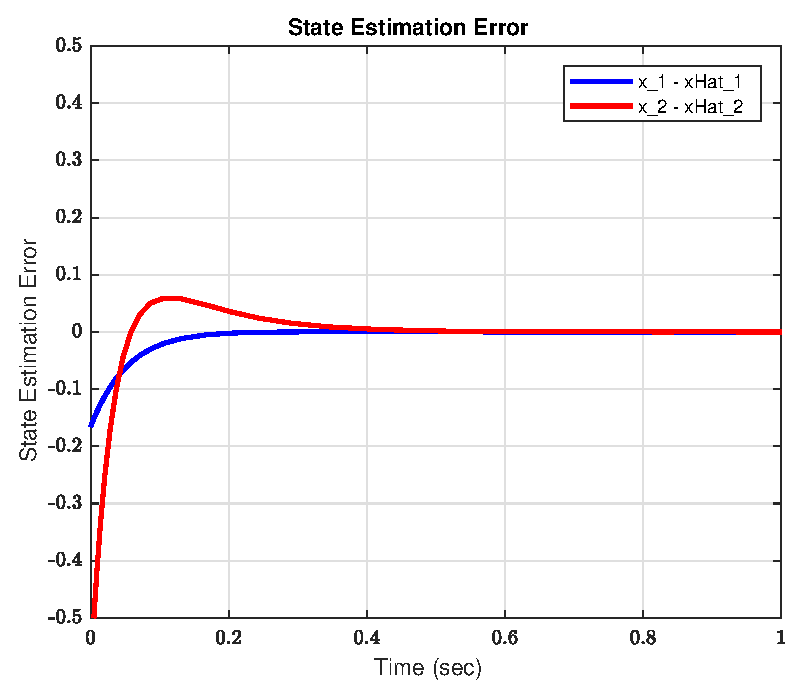
\includegraphics [width=4in]{PIO_init_02.eps}



\end{document}
    
